% Fragment prepared for insertion into the Stokes solver section of
% /Users/tgol0006/uw_folder/UW3_benchmarks/Combined_document.tex.
% It summarises pressure errors measured on curved annulus and spherical-shell
% boundaries using the benchmark-article figures.

\subsubsection{Boundary pressure error convergence}

The volume pressure norm is the primary convergence measure for the Stokes
benchmarks, but pressure errors on the inner and outer boundaries provide a
more local test of the pressure trace. This is relevant for geodynamics
applications because boundary tractions, radial normal stresses, and free-slip
or zero-slip boundary terms all depend on how accurately the discrete solution
represents pressure near curved surfaces. For a boundary
\(\Gamma \in \{\Gamma_{\mathrm{inner}},\Gamma_{\mathrm{outer}}\}\), we denote
the absolute pressure-trace error by
\begin{equation}
E_{L_2,\Gamma}(p)
=
\left(
\int_\Gamma |p_h-p^*|^2\,\mathrm{d}\Gamma
\right)^{1/2},
\end{equation}
and, where the analytical boundary pressure has a nonzero \(L_2\) norm, the
relative boundary pressure error by
\begin{equation}
E_{L_2,\Gamma}^{\mathrm{rel}}(p)
=
\left(
\frac{\int_\Gamma |p_h-p^*|^2\,\mathrm{d}\Gamma}
     {\int_\Gamma |p^*|^2\,\mathrm{d}\Gamma}
\right)^{1/2}.
\end{equation}
As in the volume pressure comparison, the pressure gauge is fixed before
evaluating errors so that the numerical and analytical pressures are compared
in the same mean-pressure convention.

The Thieulot--Puckett annulus benchmark gives a smooth manufactured solution
on a curved annulus. For the \(P_2\times P_1\) Taylor--Hood discretisation, the
inner and outer boundary pressure errors decrease close to the expected
\(O(h^2)\) trend, although the two boundaries have different error constants.
This difference is not unexpected: the inner and outer curves have different
radii, different geometric quadrature paths, and different sensitivity to the
linear approximation of the curved annulus boundary.

\begin{figure}[htb]
\centering
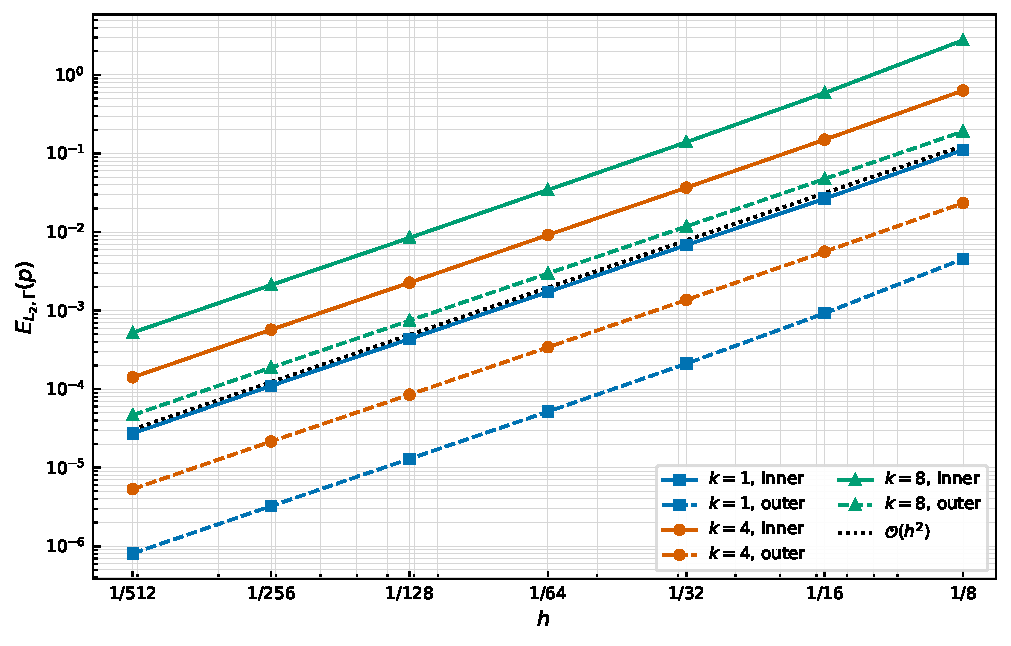
\includegraphics[width=0.82\linewidth,height=0.66\textheight,keepaspectratio]{Figures/figure_p2p1_boundary_pressure_convergence.pdf}
\caption{Absolute boundary pressure error convergence for the
Thieulot--Puckett annulus benchmark using the \(P_2\times P_1\)
discretisation. Solid curves denote the inner boundary and dashed curves
denote the outer boundary.}
\label{fig:combined_boundary_pressure_thieulot_annulus}
\end{figure}

The Kramer annulus benchmark separates smooth volumetric forcing from
delta-function forcing on an internal circular interface. The boundary
pressure errors converge close to second order for the smooth cases. The
delta-function cases also show stronger boundary pressure convergence than the
corresponding volume pressure norm because the reduced regularity is localized
at the internal interface rather than on the annulus boundaries.

\begin{figure}[htb]
\centering
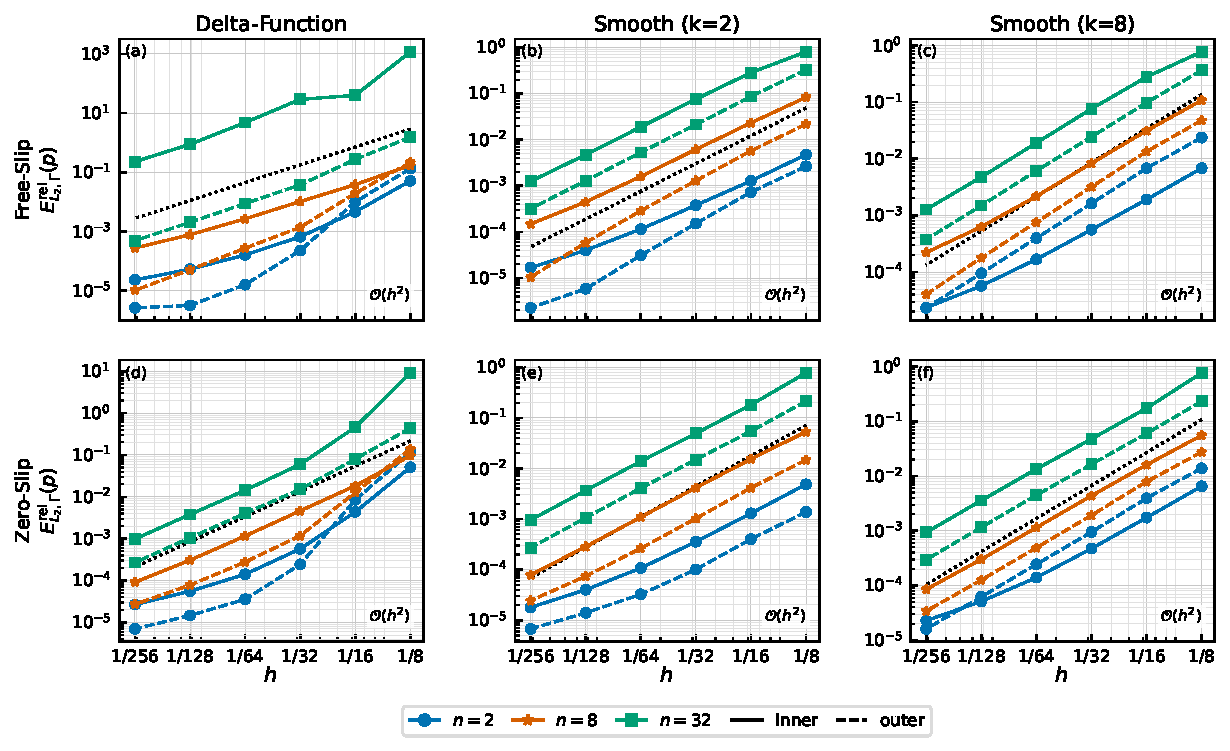
\includegraphics[width=0.95\linewidth,height=0.78\textheight,keepaspectratio]{Figures/figure_boundary_pressure_convergence.pdf}
\caption{Relative boundary pressure error convergence for the Kramer annulus
benchmark. Solid curves denote the inner boundary and dashed curves denote the
outer boundary.}
\label{fig:combined_boundary_pressure_kramer_annulus}
\end{figure}

The Thieulot spherical-shell benchmark gives the corresponding smooth
three-dimensional test. The boundary-pressure panel shows that the absolute
pressure trace errors for both \(m=-1\) and \(m=3\) decrease systematically
with refinement. These errors are shown together with radial normal-stress
errors because the stress diagnostic combines pressure and velocity-gradient
errors at the same curved spherical boundaries.

\begin{figure}[htb]
\centering
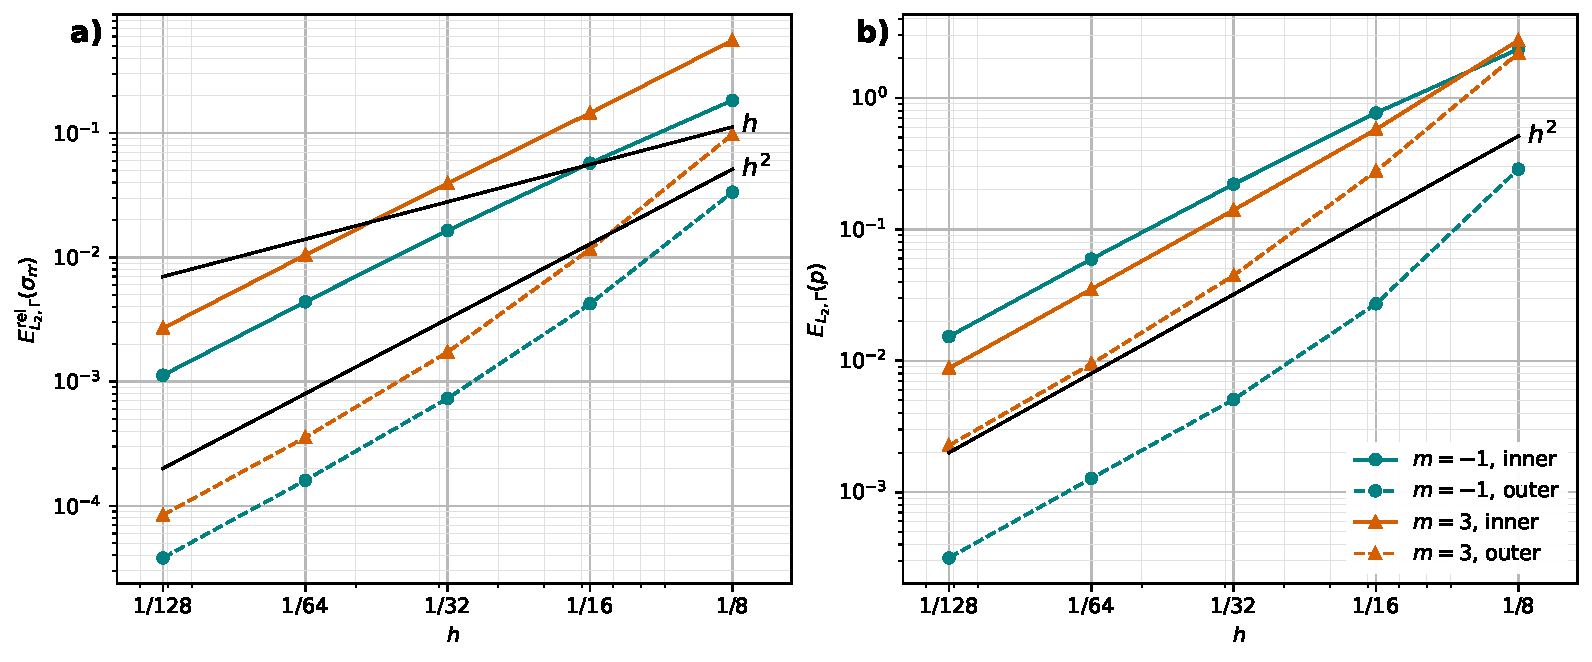
\includegraphics[width=0.95\linewidth,height=0.58\textheight,keepaspectratio]{Figures/boundary_metric_convergence.pdf}
\caption{Boundary radial normal-stress and absolute boundary pressure error
convergence for the Thieulot spherical-shell benchmark. The right panel shows
\(E_{L_2,\Gamma}(p)\) on the inner and outer spherical boundaries.}
\label{fig:combined_boundary_pressure_thieulot_spherical}
\end{figure}

For the Kramer spherical-shell benchmark, the current combined boundary figure
reports boundary velocity and radial normal-stress convergence for the
free-slip delta-function case. A boundary pressure-trace figure is not part of
the current spherical Kramer article outputs. The radial normal-stress
diagnostic is nevertheless included here because it is the closest available
boundary pressure-sensitive quantity: \(\sigma_{rr}\) contains the pressure
contribution and therefore tests pressure recovery together with
velocity-gradient recovery on the spherical boundaries.

\begin{figure}[htb]
\centering
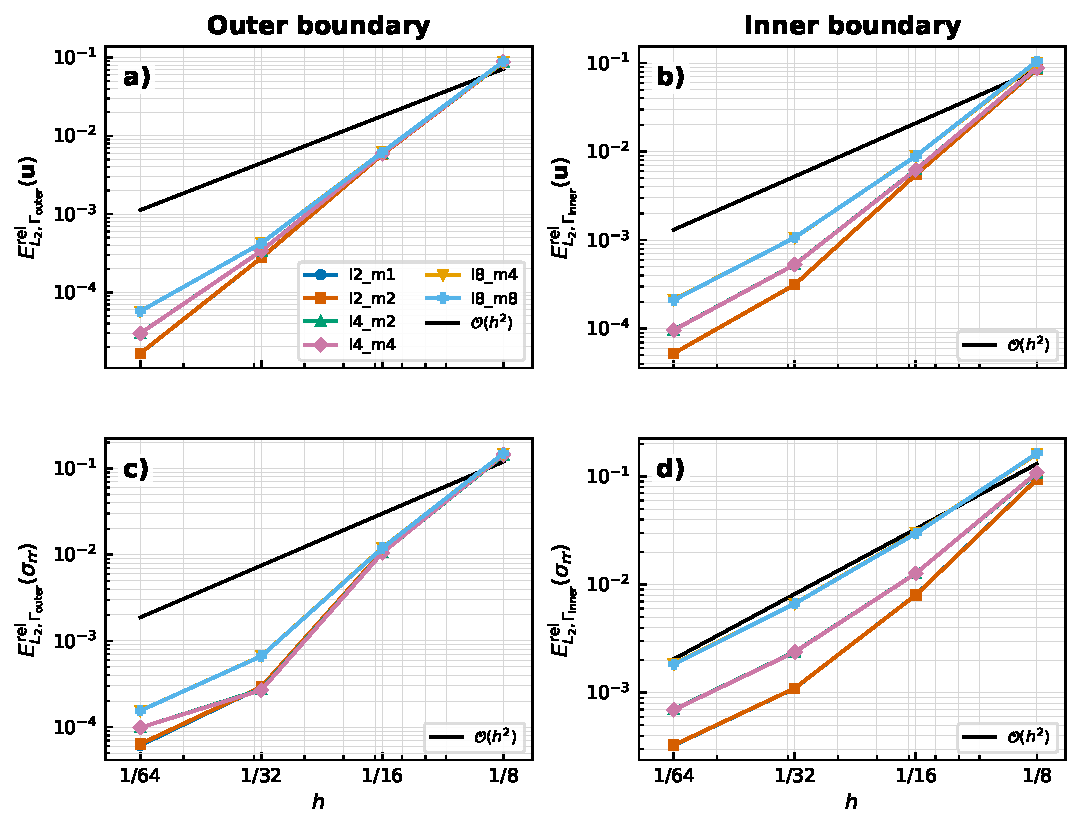
\includegraphics[width=0.82\linewidth,height=0.70\textheight,keepaspectratio]{Figures/figure_7_kramer_boundary_convergence.pdf}
\caption{Boundary velocity and radial normal-stress convergence for the Kramer
spherical-shell benchmark. This figure is included as the available
pressure-sensitive boundary diagnostic for the spherical Kramer case; the
current article outputs do not include a separate boundary pressure-trace
convergence plot.}
\label{fig:combined_boundary_pressure_kramer_spherical}
\end{figure}

Overall, the boundary diagnostics complement the volume \(L_2\)-norm pressure
errors. They isolate the pressure trace on the surfaces where boundary
conditions and stress diagnostics are evaluated. Smooth benchmark cases recover
approximately second-order pressure-trace convergence for the \(P_2\times P_1\)
pair, while singular forcing primarily affects the volume pressure norm through
reduced regularity at the internal interface. The persistent difference between
inner- and outer-boundary error constants should therefore be interpreted as a
geometric and boundary-evaluation effect rather than as a failure of pressure
normalisation.
